\chapter{Canonical Correlation Analysis}
\label{ch:methods}

%\setcounter{equation}{0}
% ==========================================================================================================

\textit{The following chapter has been adapted from:}
Wang, H.-T., Smallwood, J., Satterthwaite, T. D., Bassett, D. S., \& Bzdok, D. (2018). Finding the needle in high dimensions: A tutorial on CCA in biomedicine. Manuscript preparing for publication.
\footnote{D. Bzdok and H.-T. Wang planned the structure of the manuscript.  H.-T. Wang. drafted the manuscript under the supervision of D. Bzdok and J. Smallwood.}
% ==========================================================================================================
\section{Abstract}

Since the beginning of the \nth{21} century, the sample size of studies in medicine and neuroscience has grown rapidly. For example data sets with thousands of subjects are common and they often entail extensive neural and behavioral phenotyping yielding datasets with tens of thousands of variables. The size and complexity of these big data sets pose new challenges to researchers hoping to use them to understand relationships between brain, cognition and disease. Canonical correlation analysis (CCA) is a promising method for dealing with these large data sets. CCA allows two or more source of information to be simultaneously evaluated, such as descriptions of the brain and behavior. The present tutorial paper describes the rationale for using CCA, and considers both the promises, and pitfalls of this technique in the field of cognitive neuroscience.

% ==========================================================================================================

\section{Motivation}
\label{ch:methods:motivation}
Massive biomedical datasets and increasing computational power are opening the door to a new regime of data analysis. Similar to the advent of microarrays in genetics, brain-imaging and extensive behavioral phenotyping yield datasets with tens of thousands of variables. In the beginning of the 21st  century, the sample size of studies in medicine and neuroscience started to grow rapidly (Efron, 2010). Popularity of non-invasive brain-imaging methods provided convenient measure of brain activity and more measurement units per subject than considered participants. The advance in psychological science increased granularity of behavioral phenotypes and demographic information. For instance, UK Biobank is a prospective population study with 500,000 participants and comprehensive imaging data, genetic information and environmental measures on mental disorders and other diseases (Allen et al., 2012; Miller et al., 2016). The Human Connectome Project (HCP; van Essen et al., 2013) has recently completed brain-imaging of >10,000 young adults, with 4 hours of scanning per subject, and utilizing vast improvements in the spatial and temporal resolutions of the acquired data. The Cambridge Centre for Aging and Neuroscience (Cam-Can; Shafto et al., 2014; Taylor et al., 2017) a large (N >= 700), cross-sectional adult lifespan (18--87 years old) population-based sample designed to characterize age-related changes in cognition and brain structure and function, with raw and preprocessed brain imaging data and cognitive behavioral experiments and demographic and neuropsychological data. Extensive phenotypes and big sample size do not provide benefits without costs. Many classical statistical tools struggle to resolve datasets with more variables than observations. Moreover, the increasing data richness is accompanied with less explanatory value of a sample. The growing interest in big datasets will soon motivate researchers to seek alternative tools to ask and answer research questions in challenging rich data. 

Many classical linear-regression approaches have much contributed in the advance of neuroimaging. However, high-dimensional data were not taken into consideration when classic linear models initially designed. The present tutorial paper introduces rationale, promises, and pitfalls of one promising analysis strategy: Canonical correlation analysis (CCA). The key feature of CCA is simultaneous evaluation of two sources of detailed information, such as many brain measurements and many behavioral measurements. Two large variable sets are simultaneously co-analyzed with the capability of CCA to identify the main directions of variation in the data. CCA is an early example of multivariate statistical methods introduced in 1936 (Hotelling, 1936). However, the application of CCA has long been dormant largely due to insufficient computation power and data size. The issues once hindered the practical application of CCA were overcame, resulting in the revival of CCA in 21st century biomedicine. CCA aims not only to decompose the data into hidden sources of variation but also the correspondence between linked dimensions of two sets of variables. The possible relations between essential information from two variable sets (ie. brain and behavior) may be better reflected by the doubly-multivariate decomposition character of CCA.  In imaging and genetic neuroscience, cognition or brain function can be studied by capturing variability which does not come to the surface in a one-to-one (e.g., Pearson correlation) or many-to-one (e.g., linear support vector machines) mapping approach. With CCA’s conjoined decomposition on two variable sets, researchers can examine the hidden linear structure among various diverse variables. CCA has the capacity to yield sets of linked dimensions that explain a series of observations. The paired dimensions provide alternative views on the relations among variables. With substantially larger set of measurements and the pursuit of complex research questions, researchers in neuroscience have gained increasing interests in CCA. CCA has proven be inspirational methodology for new and continuing research (Marquand, Haak, \& Beckmann, 2017; Smith et al., 2015; Tsvetanov et al., 2016; Vatansever et al., 2017; Wang et al., 2018) with its ability to reduce the data to meaningful and concise information that allows the original experimental question to be answered. 

Our guide to CCA proceeds in four parts. We first introduce the model in details and the circumstances of use with recent applications of CCA in existing research. Next, we detail the interpretation spectrum of the CCA algorithm including limitation and pitfalls of CCA, and its similarity to other modeling technique. In closing, we provide practical suggestions of analysis.

% ==========================================================================================================
\newpage
\begin{infobox}{CCA and general linear model (GLM)}
CCA can be framed as a general example of other statistical procedures that are derived from the general linear model (GLM). Virtually all of the parametric tests most often used by behavioral scientists (e.g., ANOVA, MANOVA, multiple regression, Pearson correlation, t-test) can be subsumed by CCA as special cases in the GLM (Knapp, 1978; Thompson, 2010). Because these techniques are intricately related and fundamentally the same in many respects of CCA, learning CCA may help facilitate conceptual understanding of statistical methods throughout the GLM.
\end{infobox}

\section{Modelling intuitions}
\label{ch:methods:intuitions}
One way to appreciate the idea behind CCA is by viewing this procedure as an extension of the widely applied principle component analysis (PCA)(See Box 2.1). A principle component finds the hidden information sources that describe the biggest sources of variation among the variables. A close approximation of the original data can be reconstructed by the hidden variance source. In other words, PCA converts a set of correlated variables into a smaller number of hidden factors that were not directly observable in the original data, but effectively explain the structure of particular observation. As a prominent example, the big five personality is a psychological construct of human personality traits discovered through PCA. Personality survey data entered PCA and then finds the five hidden components that explains most of the meaningful variance of the data. The advantage of decomposition method such as PCA is its ability to reduce the original datasets to fewer and thus more interpretable dimensions. Such re-expression of the original data in a compressed, more parsimonious form has computational-statistical and interpretational appeal, while still capturing a large amount of the variability in the original large variable array. CCA maximizes the linear correspondence between linear combinations of two variable sets, similar to carrying out two PCA decompositions, but mutually linked by a joint correlation criterion. CCA reveal the two linear models describing the hidden structures. The generating process is mutually constrained by the maximum correlation of the hidden structures. Such extension of the traditional hidden factor approaches enables two sets of measurements, for example, i) genetics and behavior, ii) brain and behavior, or iii) brain and genetics. Three aspects together are characteristic for modeling data using CCA:


\begin{wrapfigure}{o}{0.4\textwidth}
    \vspace{-10pt}
    \centering
    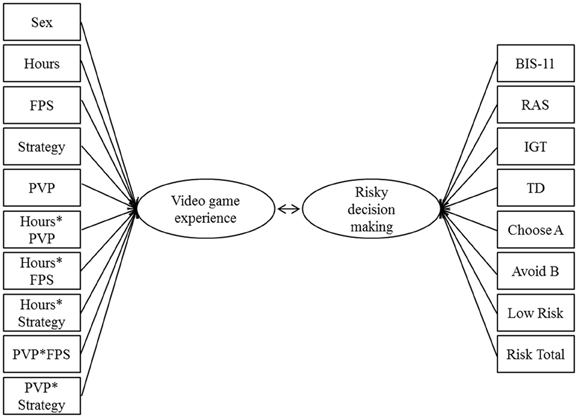
\includegraphics[width=0.38\textwidth]{cca/image/ccafig1.jpg}
	\caption{An example of CCA on behavioral data Bailey2013.}
	\caption*{Consider a case of exploring the relations between movie genre and personality with CCA. On the left hand side, we can input the data related to movies the participants watched, such as number of action / documentary / comedy etc. movies watched. The right hand side is the personality rating of the participants, for example extravert vs not, openness vs not etc. The CCA can then find the related personality traits with the type of movies they are likely to watch.}

	\label{fig:methods:fig1}
	\vspace{-20pt}
\end{wrapfigure}


\subsection{Joint information compression}
The purpose of CCA is finding variability components hidden in each of two variables sets.  The linear relations of the variable sets are determined when the variation in strength of involvement across subjects is maximally correlated. The relations to a pair of factors, their canonical correlations, indicates the conjoined explained variance across both information reductions. In a similar manner of PCA, the variables summarized the original high-dimensional variable sets with a pair of linear relations. The linear re-expression summarizes aspects of the data-generating process that was mutually constrained by the sets of input variables. The canonical correlation determines the joint explanatory power shared in the two input variable sets. CCA aims to find the most compact decomposition based on the variance explained under the contained of uncorrelated hidden dimensions. The more important components will be discovered in the earlier order.

\subsection{Symmetry}
CCA does not distinguish between the left and right variable sets during the information compression process. The canonical correlation indicates that a unit change in one component is consistently associated with an equivalent change in another component. Therefore, numerically identical decomposition results are returned regardless of the input order of two variable sets. Symmetry is a key feature that distinguish CCA from other linear regression methods. In linear-regression models, dependent and independent variables play diverging roles in the analysis. Regression indicate the impact of a unit change in the independent variable on the dependent variables, therefore dependent and independent variables cannot be exchanged to obtain an identical result. CCA, as a correlation based method, describes the co-relationship of the two variable sets, thus the exchange of the two variable sets produces identical results.

\subsection{Multiplicity}
CCA can estimating more than one corresponding component pair from the two variable sets. A pair of the components forms a mode. After finding the most important mode, CCA would then determine the subsequent linear combinations in the data patters that remain to be explained in addition to the already extracted factors. Since every new identified mode was found in the unexplained variance to the preceding mode, the modes are optimized to be uncorrelated to each other. In this manner, CCA produces a set of mutually orthogonal modes naturally ranked by explained variance. The orthogonality constraint ensues the modes each representing unique linear patterns that dominate different features in the data. When the modes are meaningful to the theory, the researchers can potentially formulate a component process approach to interpret the data.

In this way, CCA uncovers effective, symmetric linear relations that compactly summarize doubly-multivariate data. We introduced three important characteristics of CCA. First, CCA provides more effective hidden representation that capture most variance in original variables. Next, the CCA model is symmetrical in the sense that no numerical difference happens in the exchange of the two variable sets. Finally, we can estimate several modes of correspondence between the two variable sets. In the next section, we would like to explore examples of CCA applications.


\subsection{Examples}
Smith and colleague (Smith et al., 2015; see Figure 2 for the analysis pipeline) employed CCA to uncover brain-behavior modes of population co-variation in the Human Connectome Project (HCP; van Essen et al., 2013). Smith and colleague (Smith et al., 2015)aimed to discover whether any specific patterns of functional brain connectivity, on the one hand, are associated with specific sets of correlated demographics and behavior on the other hand. Functional brain connectivity was retrieved from resting state functional scans. The resting state scans measure the brain activity in the absence of a task or stimulus. 200 independent component analysis (ICA; Beckmann, Mackay, Filippini, \& Smith, 2009) networks were obtained from the resting state scans. ICA identifies all the independent networks by separating the spatial sources of the resting state data. The functional connectivity matrices were calculated based on the pair-wise correlation of the 200 networks. The behavioral measures ranging from cognitive function to demographic information entered the CCA along the functional connectivity matrices. The robustness of the modes were accessed via permutation tests on the canonical correlation. One significant mode demonstrated strong population level co-variation of network connectivity and behavioral measures. The behavioral measures spread along a positive-negative axis with intelligent, memory and cognition tests and life-satisfactory on the positive end and negative life-style measures anchoring the other end. The brain regions highly contributing to the connectivity resembles the default mode network  (DMN; Buckner, Andrews-Hanna, \& Schacter, 2008) . The positive-negative dimensions in the behavioral component and the emergence of DMN in the brain component may seem trivial on their own, however, CCA formalized the relation of the underlying biology and the correlation among the general behavioral measures that captures intelligence. Regions composing DMN has been associated with episodic and semantic memory, scene construction, and complex social reasoning such as theory of mind. The finding of Smith and colleagues (2015) strengthen the relation between DMN and high-level cognition, especially intelligence - one of the perhaps most important indices so far identified in by psychologists.

\begin{figure}[p]
	\centering
	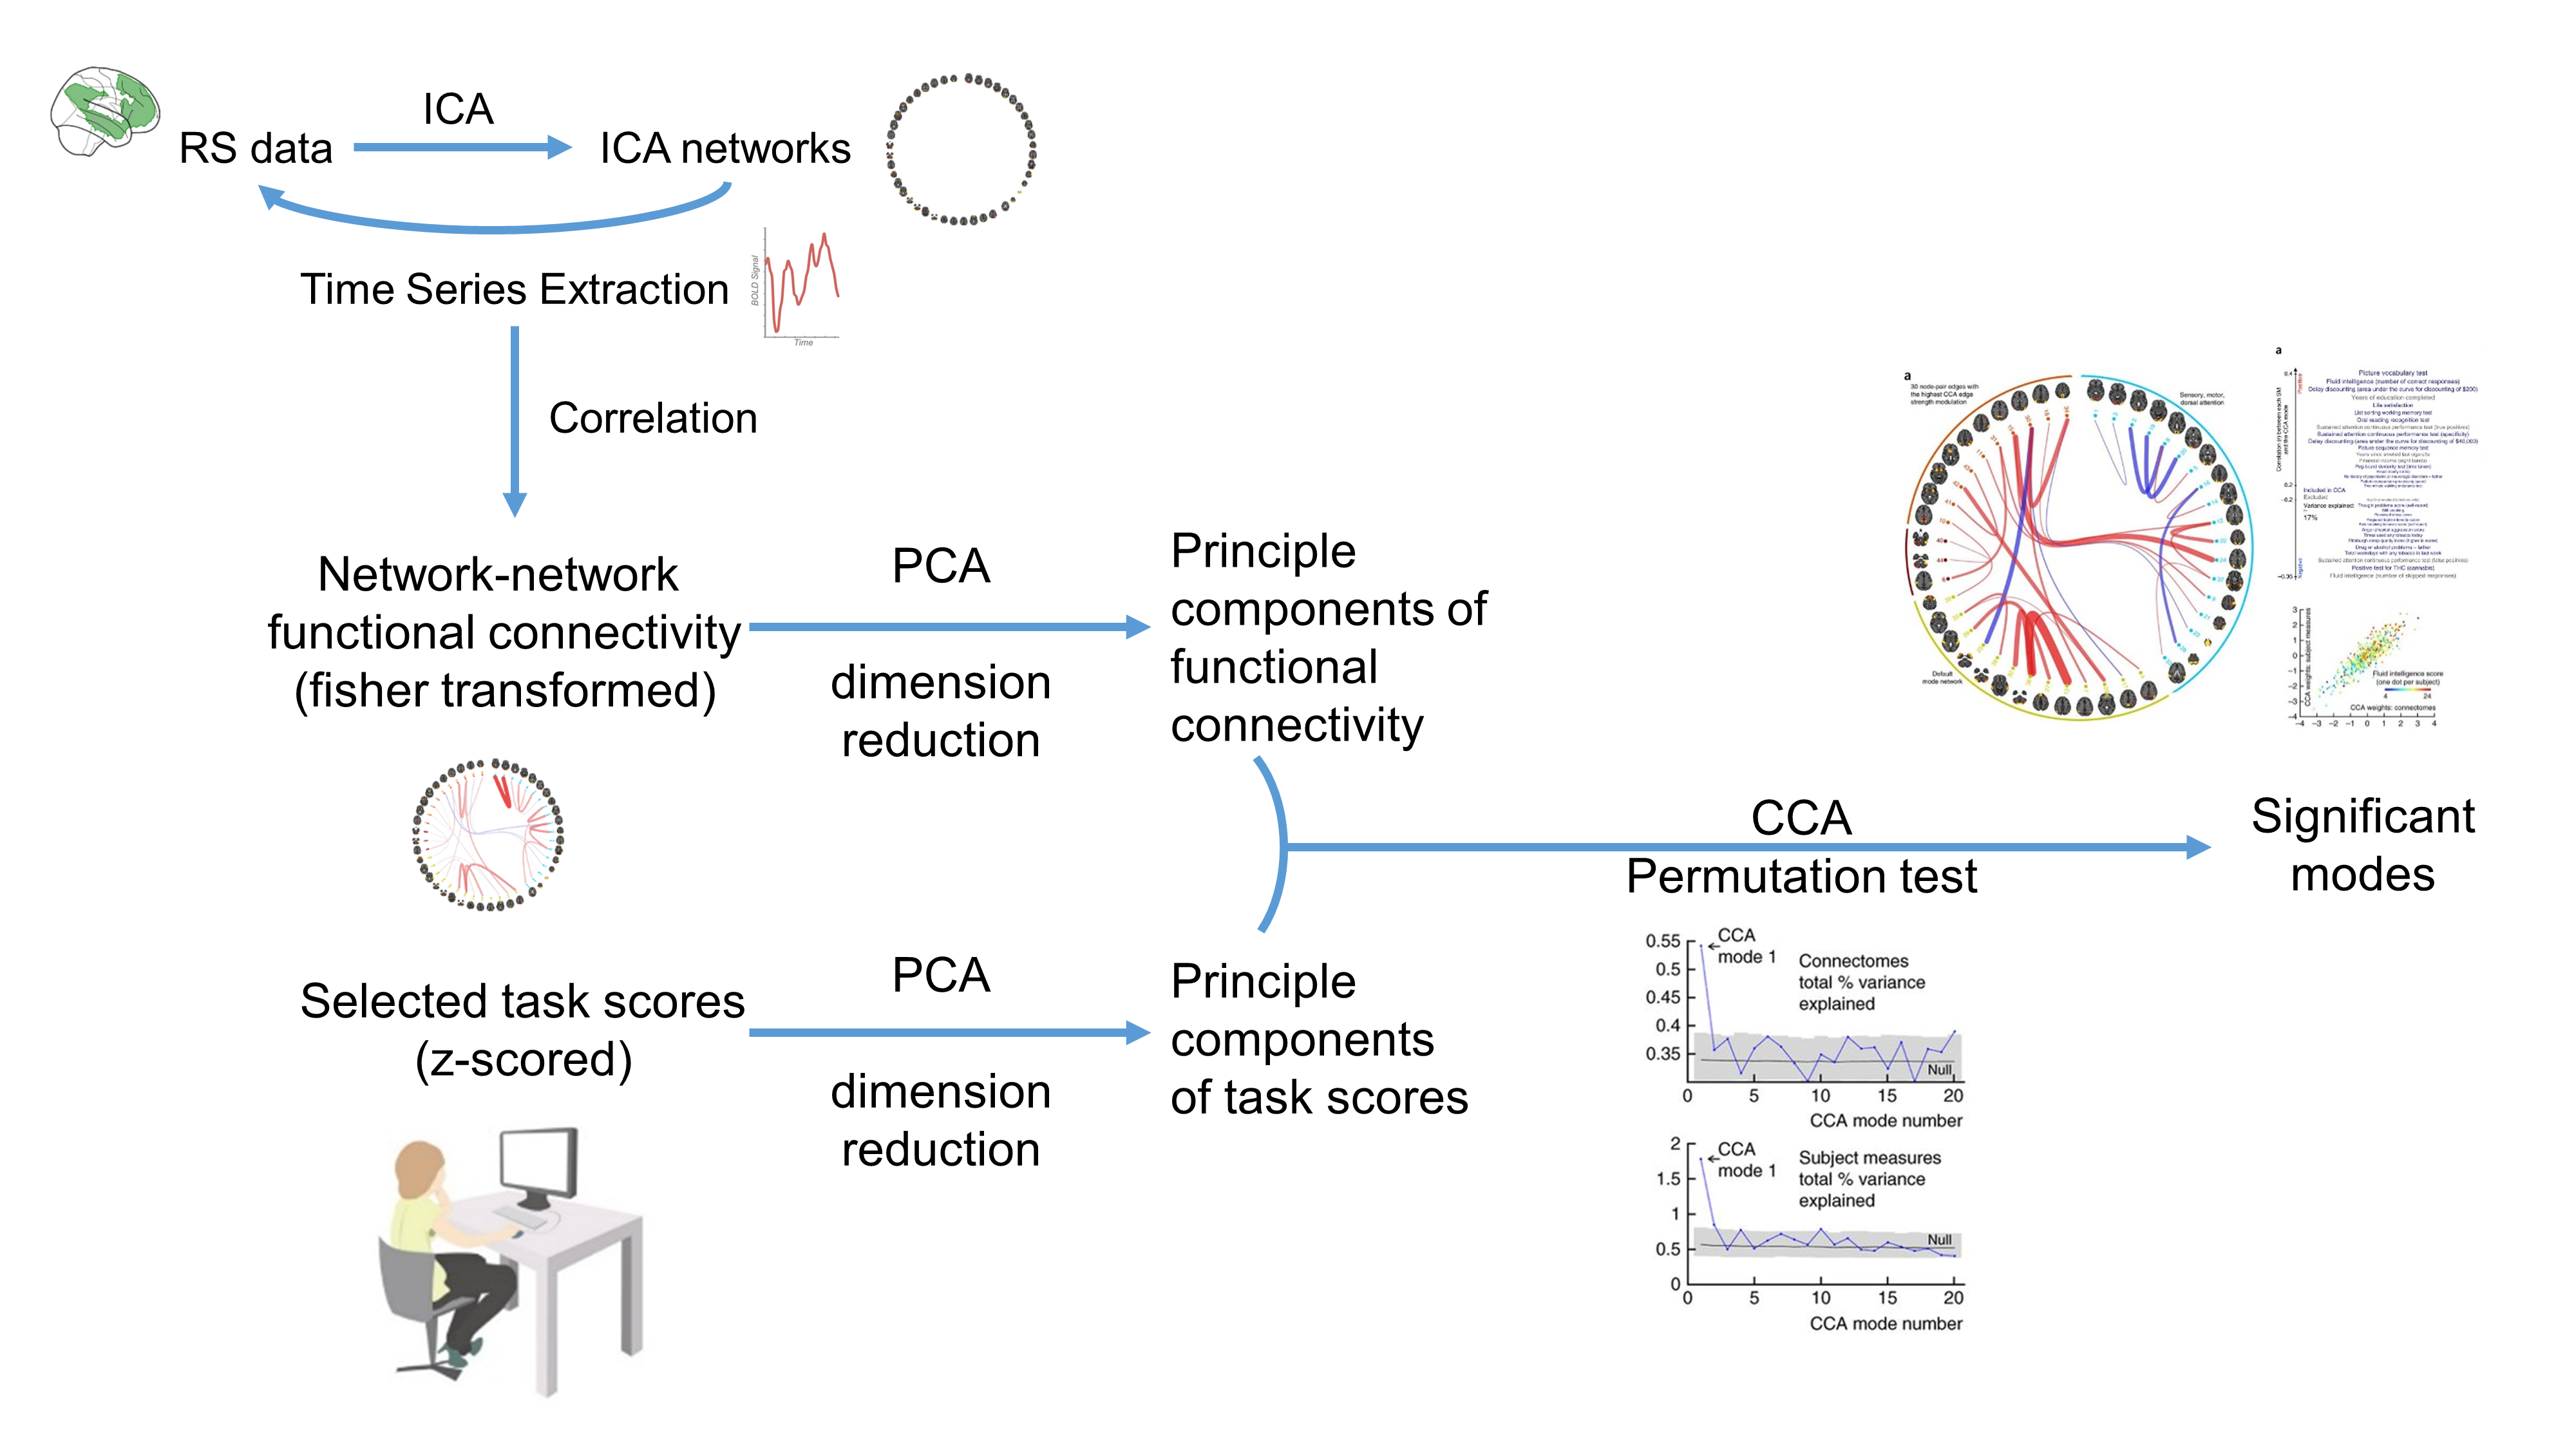
\includegraphics[width=0.8\textwidth]{cca/image/ccafig2.png}
	\caption{The analysis pipeline of Smith2015. The arrows represent analysis performed.}

	\label{fig:methods:fig2}
\end{figure}

Wang and colleagues (Wang et al., 2018; see Figure 3 for the analysis pipeline) uncover the relation between DMN and mind wandering. Mind wandering is associated with poorer performance on attention demanding tasks (McVay \& Kane, 2009; Mrazek et al., 2012), yet studies of problem solving suggest that mind wandering may promote creativity (Baird et al., 2012; Smeekens \& Kane, 2016). Despite the heterogeneity of functional outcomes, task-unrelated thoughts during mind wandering are linked to concurrent increases in DMN activity (see review from Smallwood \& Schooler, 2015). DMN is most commonly known as a task-negative network (Fox et al., 2005); however, emerging evidences suggested DMN’s role in information integration (Margulies et al., 2016). This study further explored whether the different within-DMN activation patterns underlie different types of mind wandering thought, resulting in conflicting associations to cognitive function in the mind-wandering literatures. The connectivity among 16 DMN regions and 13 self-report questions on thoughts entered the sparse variation of CCA (Witten, Tibshirani, \& Hastie, 2009). Two stable modes corresponded to traits of positive-habitual thoughts and spontaneous task-unrelated thoughts with different neural connectivity patterns in the DMN. The modes were uniquely related to aspects of cognition, such as executive control and the ability to generate information in a creative fashion, and independently distinguished well-being measures. The conflicted mind-wandering related executive failure and creativity related benefits was resolved including neural data in spontaneous thoughts decomposition. Wang and colleagues (Wang et al., 2018) showed that mind wandering is a collective term for various types of spontaneous thought. Different brain instantiations located in the DMN is the key to identify different types of spontaneous thought. The different configurations of DMN also demonstrated its possible role as an integrator in cognition, rather than a task-unrelated network.

\begin{figure}[p]
	\centering
	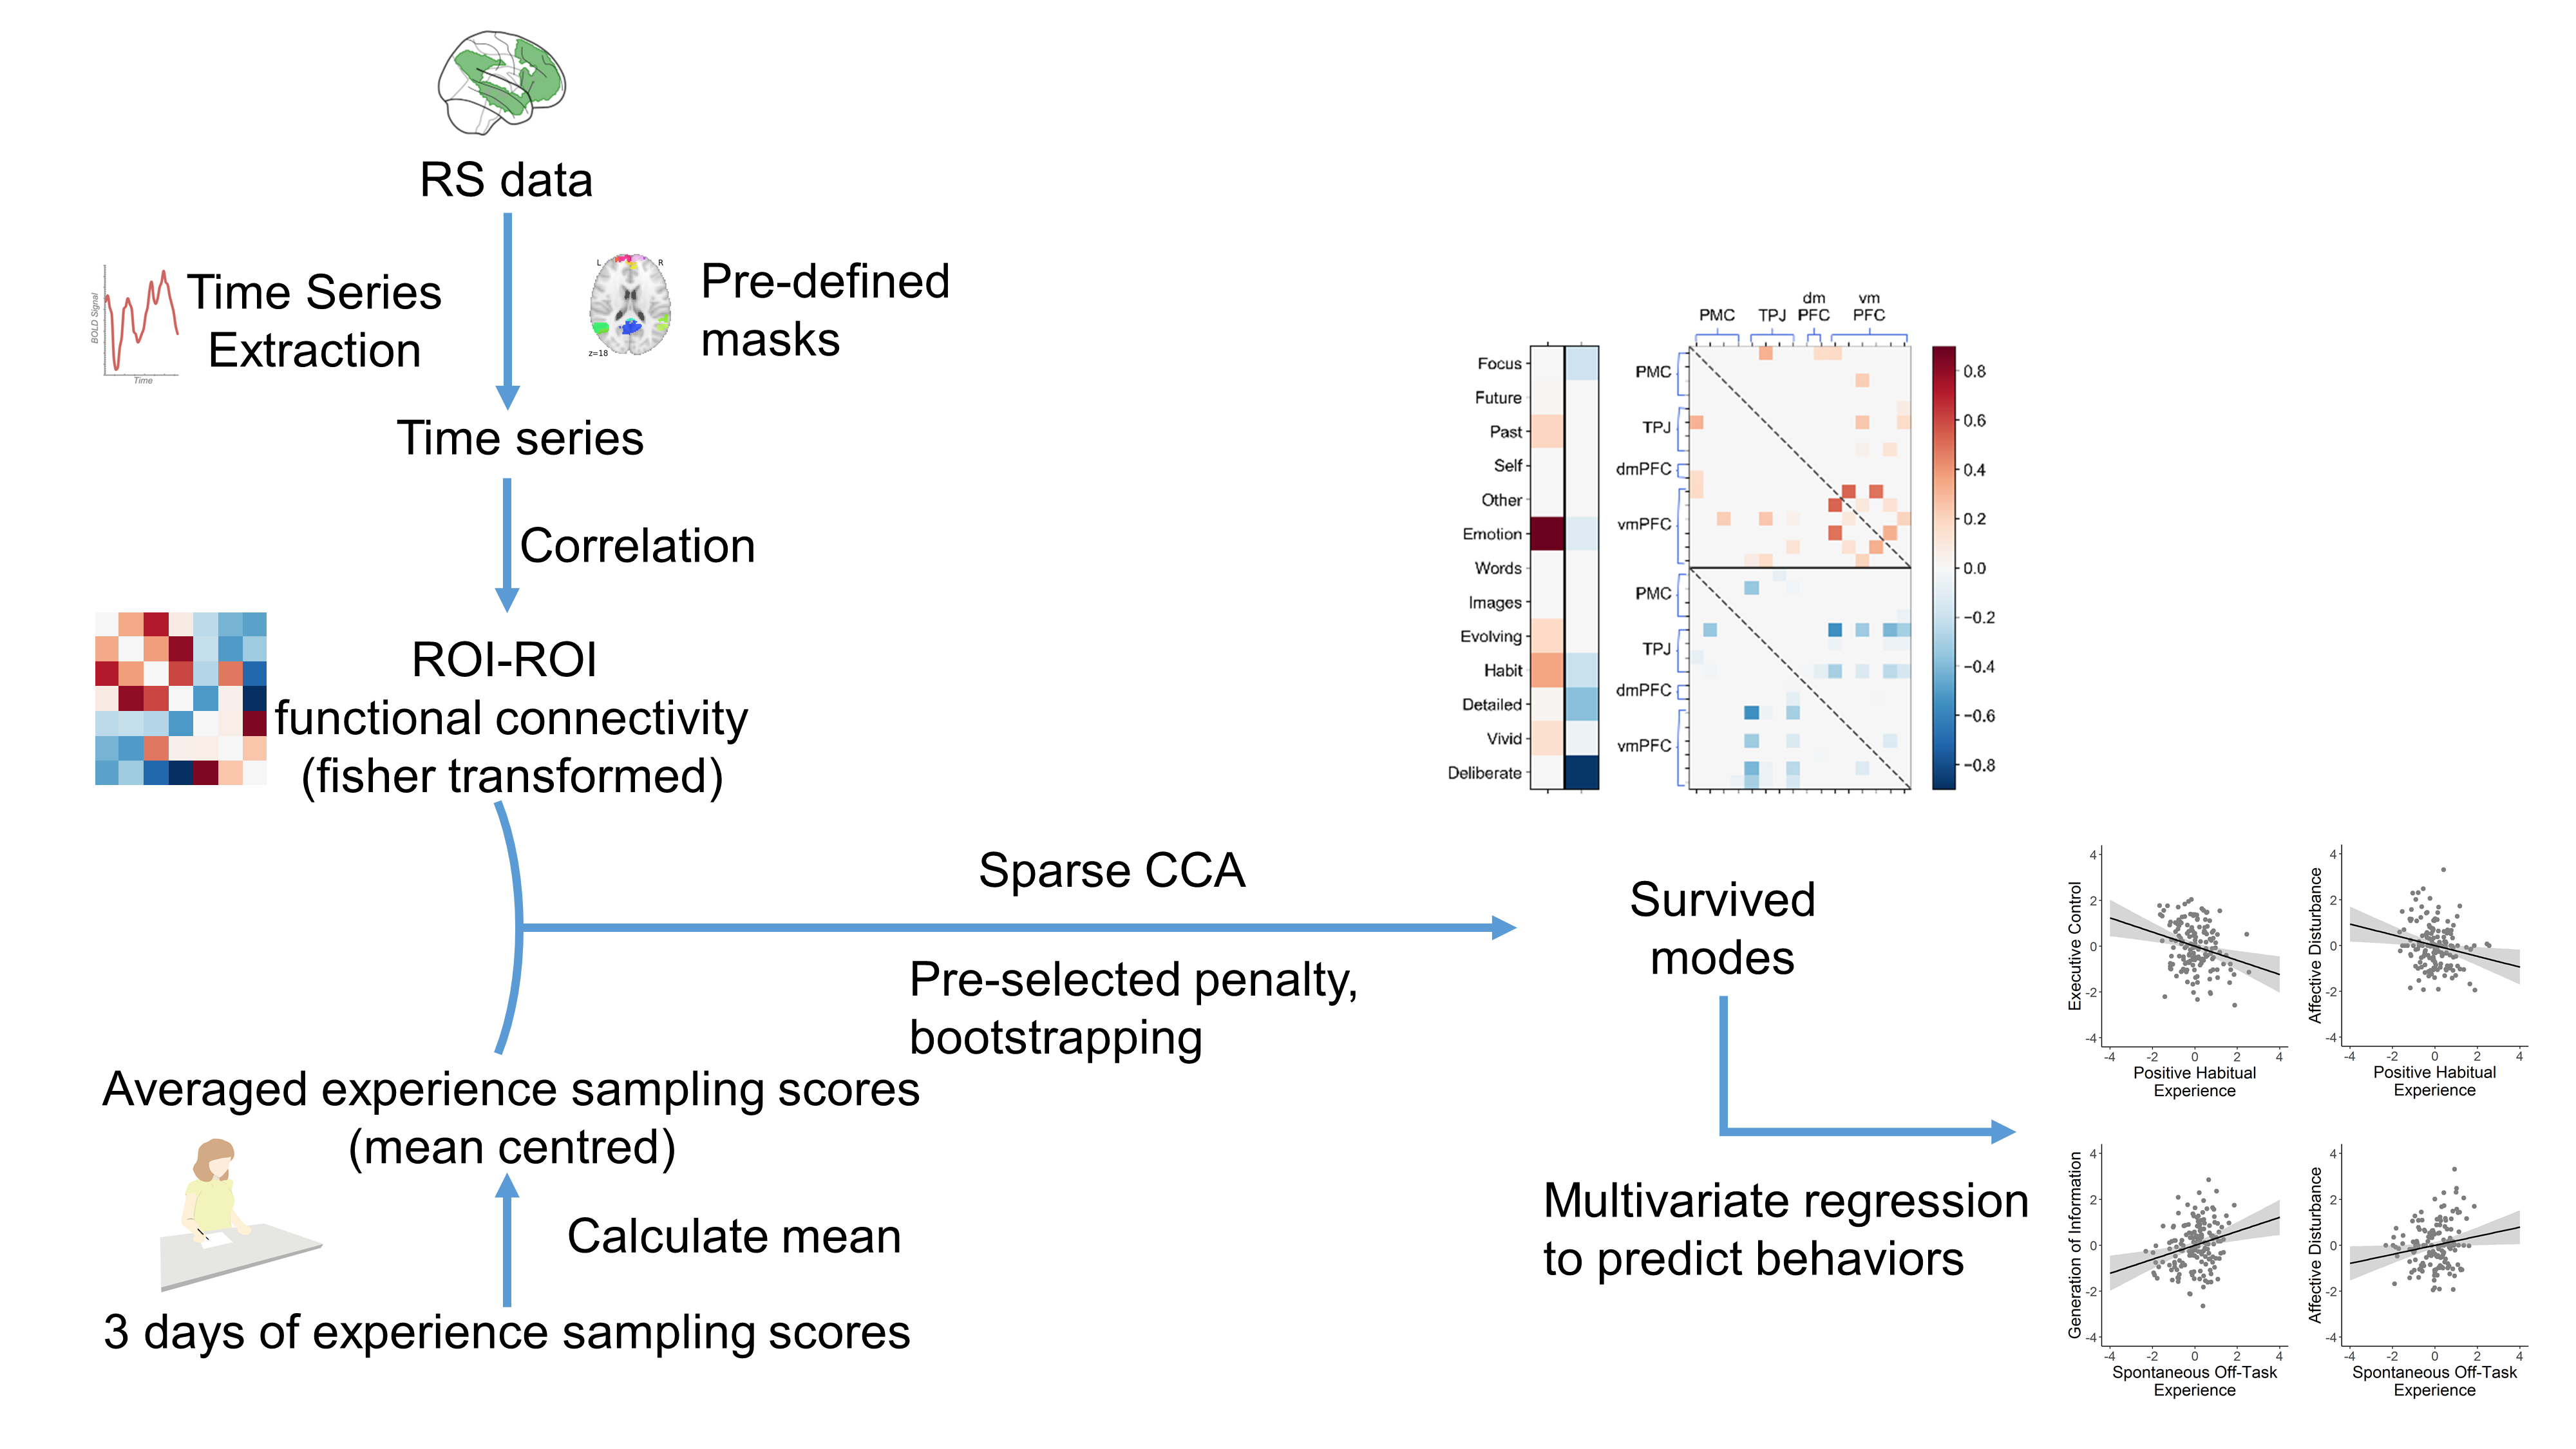
\includegraphics[width=0.8\textwidth]{cca/image/ccafig3.png}
	\caption{The analysis pipeline of WangPsychScience2018. The arrows represent analysis performed.}

	\label{fig:methods:fig3}
\end{figure}

% ==========================================================================================================

\begin{infobox}{CCA and related linear methods}

CCA is related to other feature learning methods in neuroscience. As mentioned in the modelling intuition section, \textbf{PCA} is a similar method performed on one set of variables only. The objective of PCA is a transformation of several possibly correlated variables into a smaller number of uncorrelated variables known as principal components. PCA compresses data into a smaller number of factors that carries most of the variance of the data.

\textbf{Independent component analysis} (ICA) to perform a linear transform that makes the resulting variables as statistically independent from each other as possible. The basic assumption behind ICA is that the data is composed of independent source of information. In contrast to PCA and CCA, all components are equally important.  ICA helps when you want to find a representation of your data as independent sub-elements

\textbf{Partial least squares} (PLS) regression and CCA are both techniques for feature extraction from two sets of multidimensional variables. The fundamental difference between CCA and PLS is that CCA maximizes the correlation while PLS maximizes the covariance. PLS is a supervised approach attempts to find directions that help explain both the response and the predictors. Most of the comparison between PLS and CCA are focused on the generation of the first components. There is no one way to compute the other components in PLS (De Bie et al., 2005).
\end{infobox}


\section{Interpretations}
\label{ch:methods:interpretations}
The symmetrical data compression feature of CCA helps researchers to handle the complexity of two variable sets. However, whether the process of the analysis is an exploration of hidden structures or mutually constrained predictive component has been an unsettled debate. CCA can be viewed as a supervised predictive algorithm or as an unsupervised exploratory algorithm. A supervised algorithm relies on the predefined labels/relationships in the data to form prediction; whereas an unsupervised algorithm aims to extract patterns in the data with unlabeled data. CCA has some properties of both supervised and unsupervised modeling approach. Depending on which perspective is adopted, the functions of CCA and the potential interpretation can be very different.  The more the dimensionality of one of the variable sets resembles the single output of linear-regression-type methods, the more CCA application approaches output estimation of a supervised estimator. The larger the variable sets on both sides, the more CCA approaches exploratory pattern discovery.

The main difference between supervised and unsupervised method lays in whether there is a learning target or loss function. In supervised learning, the loss function determines the best parameters to form prediction. The difference between the prediction generated by the model and the real label is the objective of a so-called loss function. CCA has as objective to maximize the linear correlation between the latent dimensions from two variable sets. While most of supervised learning methods estimates loss between real data and predictions, CCA has an unusual objective that we rarely see in supervised estimators.  Symmetry is another reason that makes CCA an unusual case of supervised learning. In supervised learning, the model learns the pattern in the data to predict a set of targets. The symmetrical nature of CCA does not distinguish the two sets of input variables. The data compression and hidden structure inspection aspect puts CCA in line with unsupervised methods. The conjoined decomposition captures the relations among the variables. The found relations are used to construct fewer factors that capture the variance of the original data. CCA has the strength of both supervised and unsupervised methods. Like unsupervised methods, CCA can search through candidate patterns to find structure in data. The accurate predictions formed by CCA highlights the trait of a supervised method. In conclusion, CCA is a special case that sits in-between the supervised and unsupervised methods. The flexibility in interpretation offers people multiple ways to utilize CCA in research.

Statistical methods can be categorized into three categories based on their goals: estimation, prediction, and inference.  Estimation represents ways or a process of learning and determining the population parameter based on the model fitted to the data. Prediction is making inference of an unknown data points based on information obtained from a sample. Inferential statistical analysis utilizes hypothesis testing to draw conclusions about populations or scientific truths from data. CCA falls into the family of estimation. The focus of CCA is to establish statistical associations (i.e. the latent linear relations among variables, the association between the two latent linear relations). Predicting some variables based on other variable is not the optimization goal. CCA does not seek to establish “statistically significant links between variables”. The null hypothesis that is really tested around the robustness of the latent space correlation (i.e., the canonical correlations of the latent variables extracted from the two variable sets) across modes, not so much particular variable-variable links. CCA is often used to rigorously evaluate whether overall linked covariation patterns can be found in two variable sets, rather than pinpointing and “putting the finger on” certain specific relations that should be interpreted with more caution.

\begin{figure}[p]
	\centering
	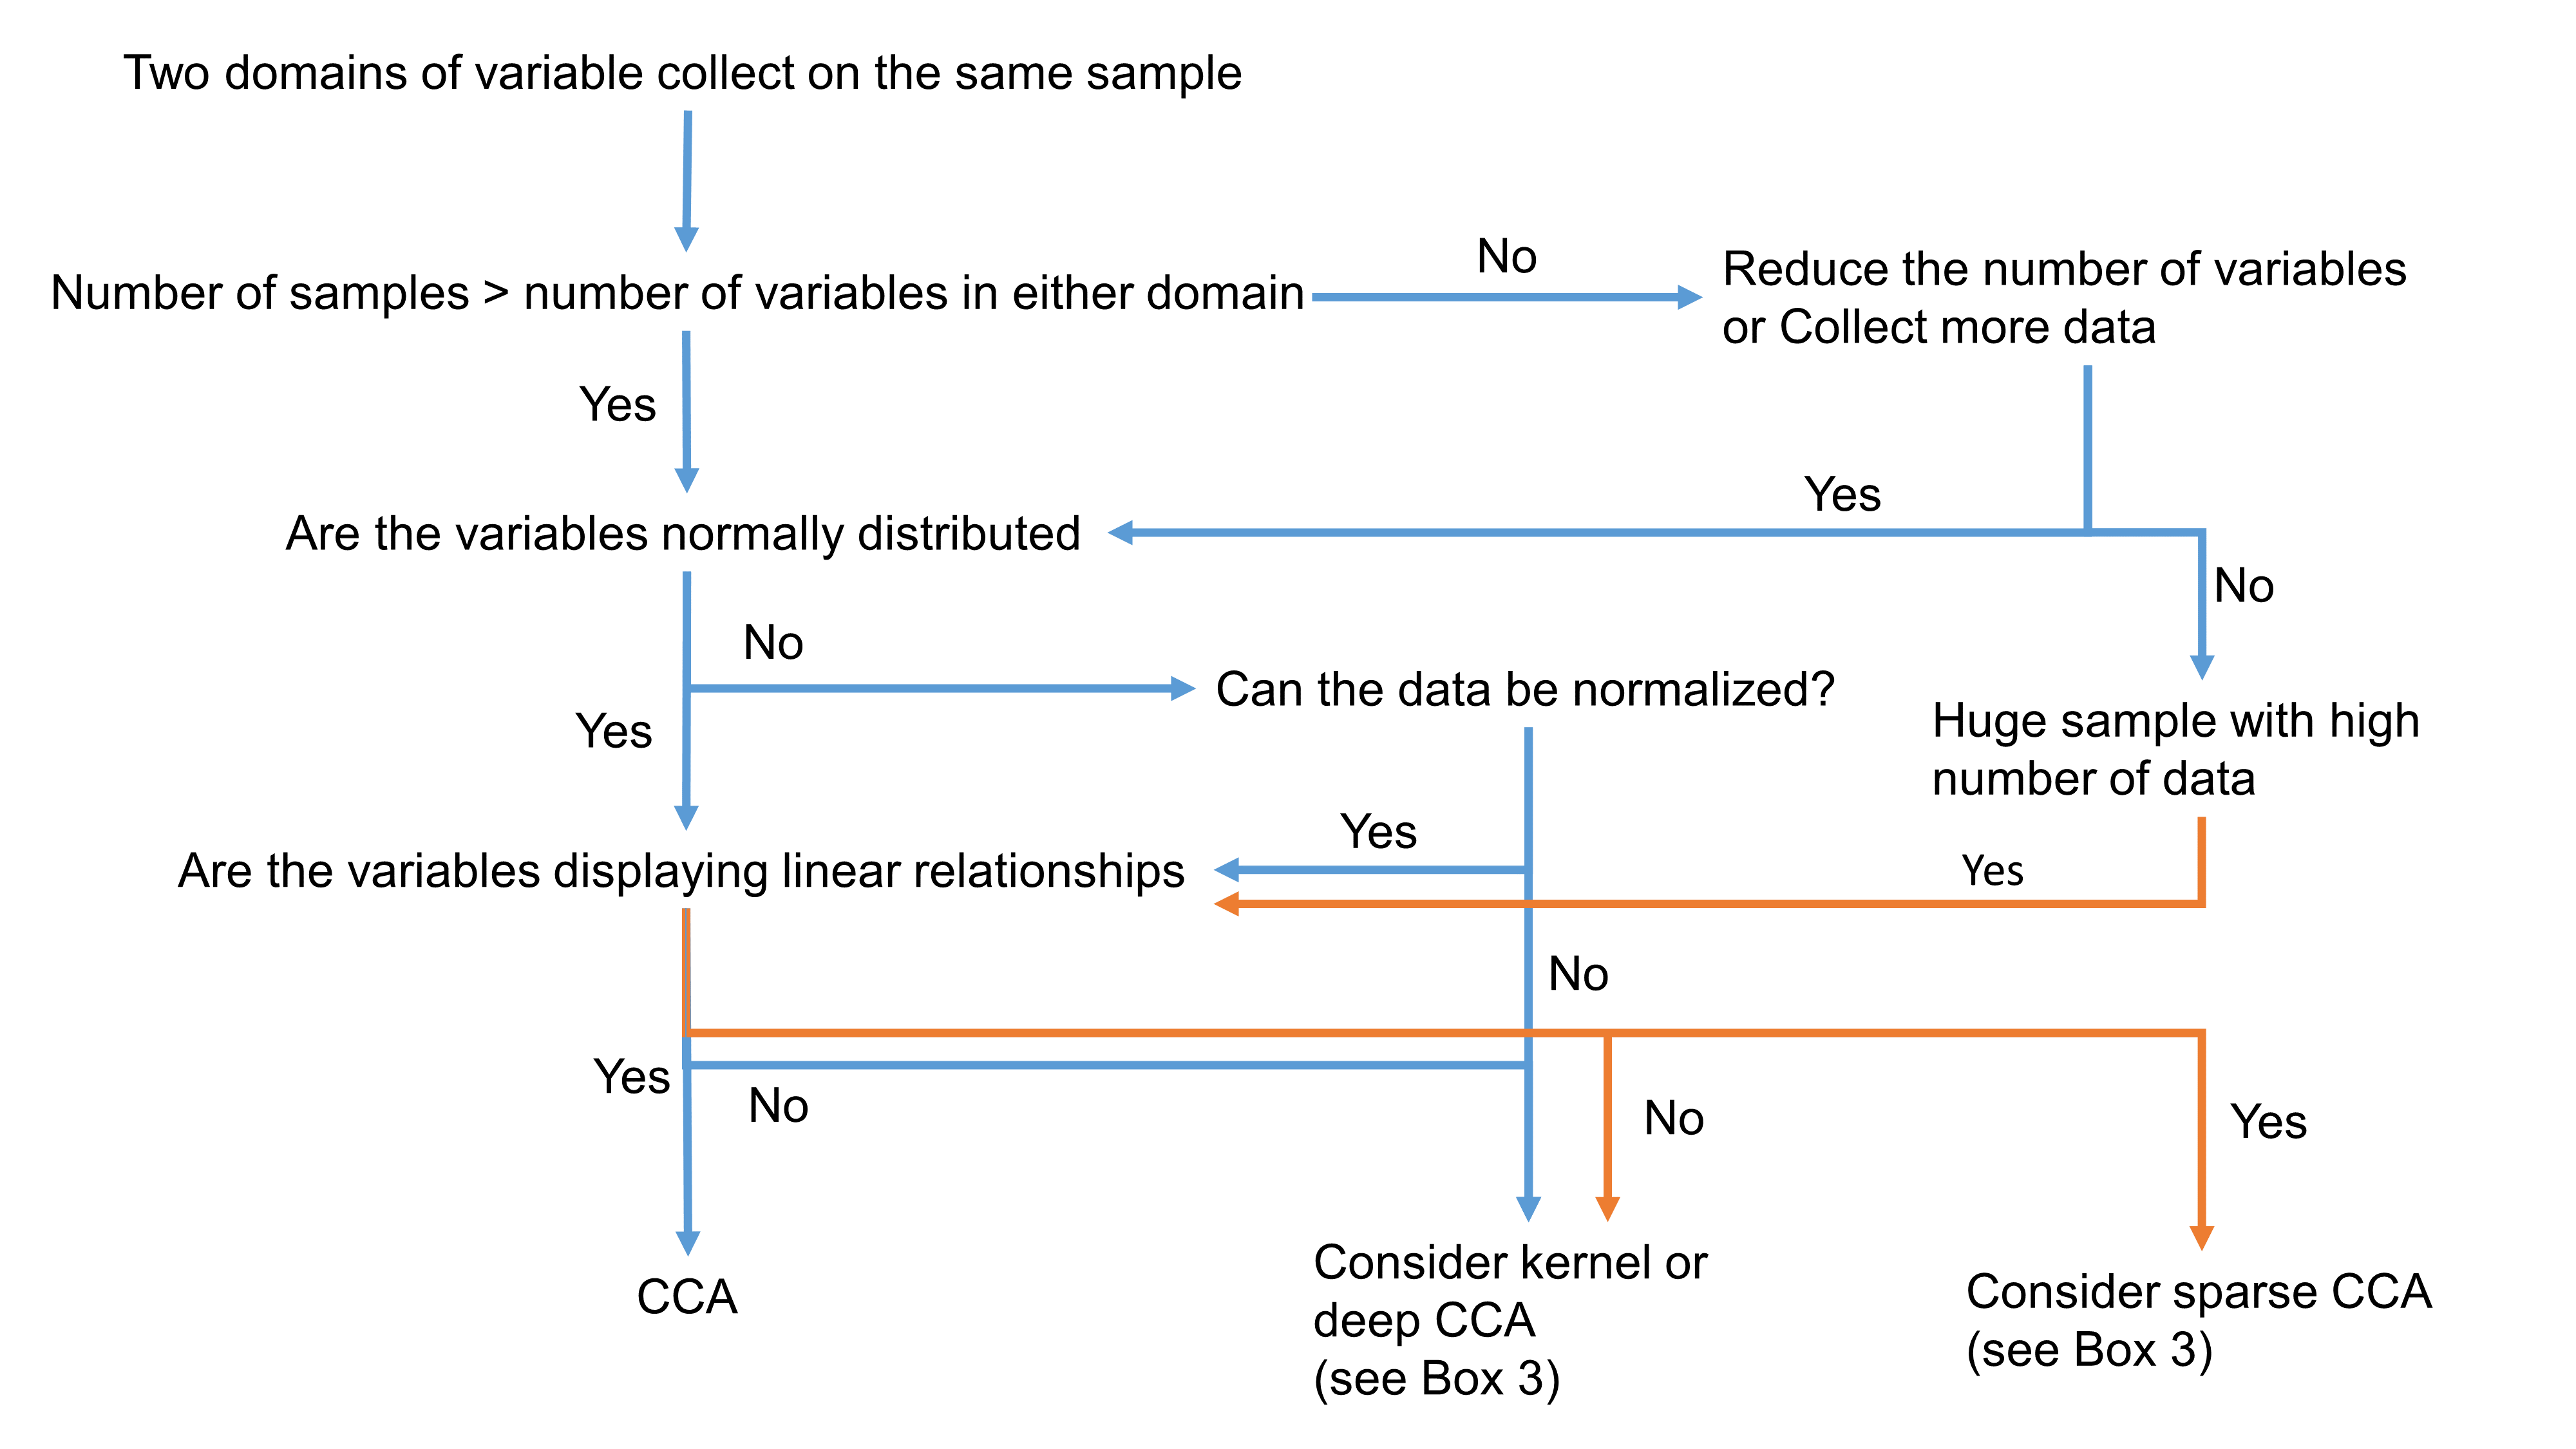
\includegraphics[width=0.8\textwidth]{cca/image/ccafig4.png}
	\caption{A flow chart illustrating the choices when considering the application of CCA to a data set.}
	\label{fig:methods:fig4}
\end{figure}

% ==========================================================================================================

\subsection{Limitations}
\label{ch:methods:limitations}
The strength and benefit of CCA do not come without limitations. Here we discuss several aspects the researchers should keep in mind when evaluating whether the data set is suitable for CCA. CCA can handle data with more observations than number of variables of the smaller variable set (i.e. p < min(m, n)). However, smaller dataset does not fully utilize the strength of CCA in concluding the variability in data. Research areas like neuroscience often look into small effect magnitude in correlation, thus a larger sample size is required to correctly infer the variability in data. On the other hand, if the number of variables of either side of the equation exceeds the sample size, CCA does not generate unique linear combinations for each variable set.  In such scenario, a PCA rank-reduction preprocessing step is commonly performed before applying CCA. 

The structure of CCA is essentially a linear model, hence some limitations stem from the assumptions of normality and linearity. CCA can accommodate any metric variable without the strict assumption of normality. However, normality is desirable because it allows for the highest correlation among the variables. It is highly recommended to evaluate the normality of all variables and apply data transformation if possible. CCA uncover the linear relationships among the variables of interest. The linear assumption introduces two limitations to CCA. Firstly, since only linear effects can be captured, non-linear effects will not be captured. Data transformation or alternative CCA variation would be the solutions (see Relation to other commonly used methods). Secondly, the optimization objective is about correlation in CCA (i.e. see Interpretation). The discovered relationships are not necessarily accurate predictions in future data. Any interpretation and application related to predictability of the canonical components should be treated with caution. 

\begin{infobox}{Overcoming the limitations of linear CCA}
Several useful extensions of CCA has emerged in the past decade to overcome the limitation of the linear version of CCA. The first was the nonlinear version of CCA, with \textbf{kernelization of CCA} (KCCA; Hardoon et al., 2004) as the representative.  Kernels are methods of implicitly mapping data into a higher-dimensional feature space with kernel function, a method known as the kernel trick. KCCA first project the data into a higher-dimensional feature space before performing CCA in the new feature space.  While KCCA allows learning of nonlinear representations, the drawback is that the representation is limited by the fixed kernel. KCCA is a nonparametric method, hence, the time required to train KCCA or compute the representations of new data points scales poorly with the size of the training set.

\textbf{Sparse CCA} (SCCA; Witten \& Tibshirani, 2009) is a method for identifying sparse linear combinations of the two sets of variables that are highly correlated with each other. It has been shown to be useful in the analysis of high-dimensional data, when the variable number of either arrays is higher than the number of samples. The sparse feature reduces the some coefficients to 0 in the linear structure depending on the penalty parameters. The benefit of sparsity is improvement in interpretation and feature selection. However, sparsity violates the orthogonality of CCA, meaning the components in different modes can correlate with each other. The explained variance of each mode will not follow the rank order either. Recently, we have used k-fold cross validation to identify the ideal level of sparsity in a study that explores the relationship between patterns of thought at rest and the associated brain organization (Wang, Bzdok et al., 2018).

With the recent advance in deep neural network, \textbf{deep CCA} (DCCA; Andrew et al., 2013) has been proposed as an alternative to KCCA as a non-linear method for CCA. Deep neural network is an algorithm that learns the representation of data through multiple non-linear transformations. The name came from the architecture that loosely follows the connections of neurons. DCCA simultaneously learns two deep neural network mappings of two variable sets that are maximally correlated. The main advantage is the faster performance over KCCA, because DCCA directly learns the data without re-mapping data into a higher dimension. 
\end{infobox}





% ==========================================================================================================


\section{Practical considerations}
\label{ch:methods:impliment}

Having introduce the features and interpretations of CCA, we would like to arise some practical considerations for the implementation. The computation of CCA is available in the in-built library of MATLAB (canocorr) and R (cancor), and Python machine-learning library scikit-learn (sklearn.cross\_decomposition.CCA). All implementations above provides comprehensive documentation of the basic usages. In the current section, we would like to mention details and problems that might happen while performing CCA on real data.

\subsection{Preprocessing}
Some minimum data preprocessing is required due to the linear nature of CCA. The objective of CCA is maximizing correlations. The nature of correlation is defined by the simultaneous unit change of the two variables; therefore, the computational process has implicitly standardize the data. The features obtained from CCA are therefore scale invariant.  (cf. PLS optimizes the covariance; therefore, the output will be influence by scaling.) Scaling, such as z-transformation, is still recommended before performing CCA for the ease of interpretation. This helps people to focus on unit chance rather than absolute values of data. Linear relationship is sensitive to outlier effects. To avoid outliers skewing the results, replacing outliers with mean or median is highly suggested. Aside from outliers, some confound variables can also introduce unwanted effects. Confound variable removal is recommended as a preprocessing step to reduce the risk of finding non-meaningful associations. To perform confound removal, we can fit a linear regression composed of the confound variables on each of the variables. The residual would be the variable without influences of the confounds.  

When the number of variable exceed the number of sample, PCA is recommended as a dimension reduction step before the analysis. An example is the work by Smith and colleague (2015). The downside of this method is that we cannot directly map the result to the original data. To interpret the CCA solutions in the original data, Smith and colleague (2015) correlate the canonical variates to the original data to recover the relevant variate captured by the CCA component pair. 

CCA component can be ambiguous for interpretation, especially when a PCA dimension reduction is applied. An alternative solution is a  CCA+ICA method (Miller et al., 2016; Sui et al., 2010) has been proposed to overcome the issue of projecting the PCA-compressed back to the original space. In the original CCA+ICA approach, the assumption is that CCA extracted components are an incomplete decomposition with multiple possible source (i.e. patients vs controls). CCA first finds the correlated variance of the two variable set. After CCA, the canonical components are concatenated into one array. ICA is then applied to the canonical components to recover the source of the variance. The ICA step can be done in the full feature space by projecting the CCA components to the PCA components (Miller et al., 2016). The CCA+ICA approach achieves both high estimation accuracy and to provide the correct connection between two variable sets. The ICA step is especially useful in detection of independent components that contribute to the common solution extracted from the two variable sets. 

\subsection{Model selection}
To select the number of mode (canonical component pair, see 3.3 Multiplicity), we can use explained variance to determine the final number of modes. The calculation can be done by predicting the canonical components with the original score with a linear regression. Another solution is to calculate the family-wise error rate through permutation tests.  The permutation is done on one of the variable sets, and then perform CCA on the permuted null sample. The first canonical correlation of the null sample is compared with all the CCA modes extracted from the real data. The p-value for each mode is calculated as number of null canonical correlation higher than the given mode from real sample, divided by  the number of permutation.
The variations of CCA might need an extra step for hyperparameters selection, such as kernel type and penalty in KCCA, penalty in SCCA, and layer number in DCCA. A permutation or cross-validation scheme is recommended for hyperparameters selection. The permutation test on hyperparameter selection is set up in the same way as model selection, but focusing on the first canonical correlation only (For example, see Appendix A in Witten \& Tibshirani, 2009). In terms of cross-validation, the objective function for model selection can be the out-of-sample explained variance or the variance loss between the training set and the testing set. 

% ==========================================================================================================
\section{Summary}
\label{ch:methods:summary}
CCA is a doubly multivariate pattern analysis on two variable sets. With no directionality implied on either variable set, CCA enables more flexibility on the research questions. As the interest in multitask data and rich cognitive phenotyping in large dataset grows, CCA fulfills the need of a method that considers all possible variables in one analysis. With its ability to reduce the data to meaningful and concise information, CCA is a promising method for scientists who are interested in exploration of multivariate patterns in large data sets.